\documentclass{article}
\usepackage[utf8]{inputenc}
\usepackage[english]{babel}
\usepackage{graphicx}
\usepackage{amsmath}
\graphicspath{ {images/} }

\begin{document}
% Title page
\begin{titlepage}
    \vspace*{\stretch{1.0}}
    \begin{center}
        \Large{Udacity Machine Learning Nanodegree Capstone}\\
        \LARGE\textbf{Quora Duplicate Question Detection}\\
        \vspace{1cm}
        \large\textit{Raahul Seshadri}\\
        \normalsize{April, 2017}
    \end{center}
    \vspace*{\stretch{2.0}}
\end{titlepage}

% Table of contents
\tableofcontents
\newpage

% Begin sections
\section{Definition}

\subsection{Project Overview}
Websites like Quora\footnote{https://www.quora.com}, StackExchange\footnote{https://stackexchange.com} network (includes the popular programming website StackOverflow) allow the users to post questions, and the entire community can answer those questions. Ideally, every unique question should be present just once in the system, so that every answer to those questions are present at once place.

However, users are prone to posting duplicate questions, because not all of them check if the question they're asking has already been asked by someone else. This necessitates having an automated duplicate question checker that can check if a question is a duplicate. Whenever the user tries to post a new question, the system can suggest an existing one for perusal.

This project was inspired by Quora's Kaggle challenge\footnote{https://www.kaggle.com/c/quora-question-pairs}. A dataset of question pairs, manually tagged as duplicate or note, has been provided by Quora to train on.

\subsection{Problem Statement}

The problem can be stated as follows:

\begin{center}
\textbf{Given a question pair, detect if they are duplicate or not.}
\end{center}

The steps to achieving our duplicate detector are as follows:

\begin{enumerate}
\item{Download and pre-process the Quora training dataset}
\item{Split the Quora training dataset into 90\% training and 10\% test set.}
\item{In the 90\% training set, further 10\% will be used as a validation set.}
\item{Extract usable features from the dataset.}
\item{Train a binary classifier to differentiate between duplicates/non-duplicates.}
\item{Provide a command-line interface so that users can check for duplicates from Quora's test set, or provide his own questions.}
\end{enumerate}

\subsection{Metrics}

Being a classification problem, the metric is going to be accuracy:

$$\text{accuracy} = \frac{\text{true positives} + \text{true negatives}}{\text{total samples}}$$

This accuracy will be measured on the test set (10\% of the total dataset).


\section{Analysis}

\subsection{Data Exploration}

Let's look at how the Quora dataset is structured:

\noindent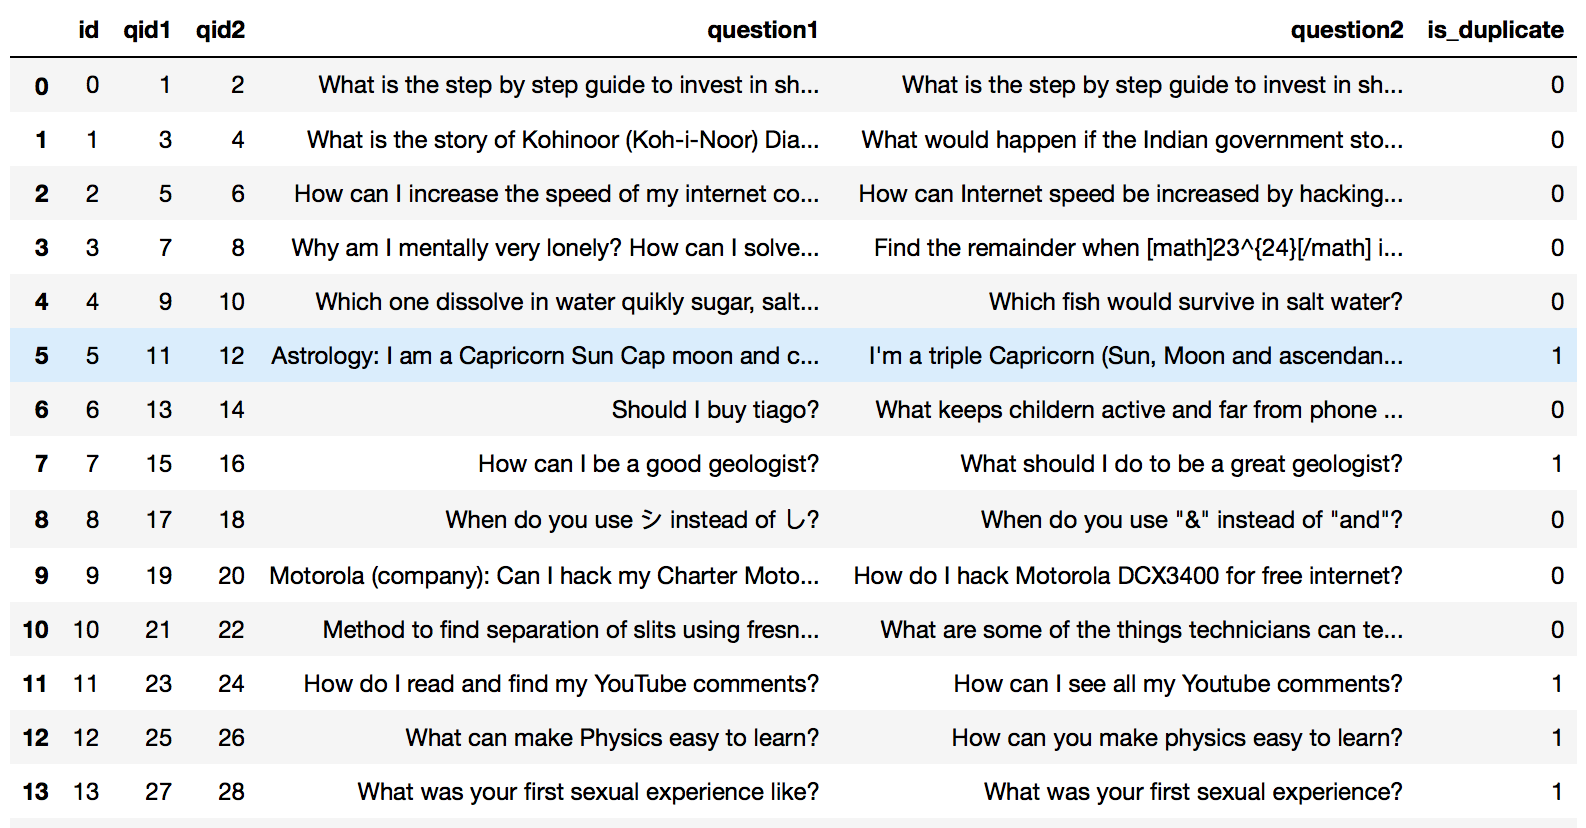
\includegraphics[width=\textwidth]{data_head}

\end{document}
